\section{Durchführung des Versuches}
\label{sec:Durchführung}

\subsection{Aufbau des Versuches}
\label{subsec:aufbau}
Der schematische Aufbau des Versuches ist in Abbildung~\ref{fig:aufbau}
dargestellt.
\begin{figure}[H]
  \centering
  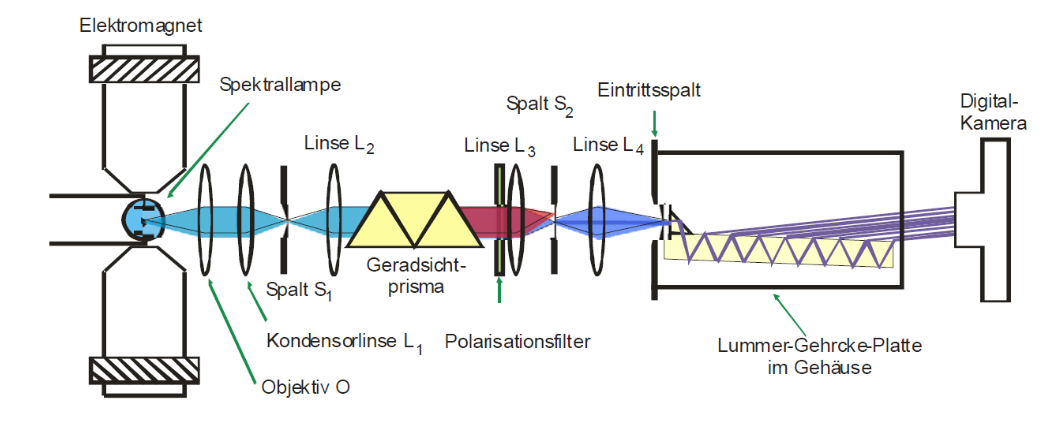
\includegraphics[scale=0.4]{pictures/aufbau.png}
  \caption{Schematischer Aufbau des Versuches. \cite{Versuchsbeschreibung}}
  \label{fig:aufbau}
\end{figure}
\noindent
Durch eine Cadmium-Spektrallampe wird ein Cadmium-Spektrum erzeugt. Die
Lampe steht zwischen den Polschuhen eines Magneten, welcher aktiviert
werden kann, damit die Aufspaltung des Spektrums in Magnetfeldern beobachtet
wird. Ein Geradsichtprisma spaltet die Emissionslinien nach ihrer
Wellenlänge auf. Durch einen Spalt können einzelne Linien des Spektrums
untersucht werden. Durch einen Polfilter wird die Polarisierung gewählt.
Eine Lummer-Gehrcke Platte wird verwendet, um die Auflösung zu
erhöhen. Das Interferenzmuster der Lummer-Gehrcke Platte wird mit einer
Digitalkamera aufgenommen.

\subsection{Die Lummer-Gehrcke Platte}
\label{subsec:lummergehrcke}
Eine Lummer-Gehrcke Platte besteht aus mehreren planparallelen Platten, welche
dazu genutzt werden, um über Interferenz eine Messung der Wellenlänge in die
Messung des Gangunterschiedes umzuwandeln. Dies kann mit sehr hoher
Genauigkeit erfolgen. In Abbildung~\ref{fig:lummergehrcke} ist der Strahlengang
in der Platte dargestellt.
\begin{figure}[H]
  \centering
 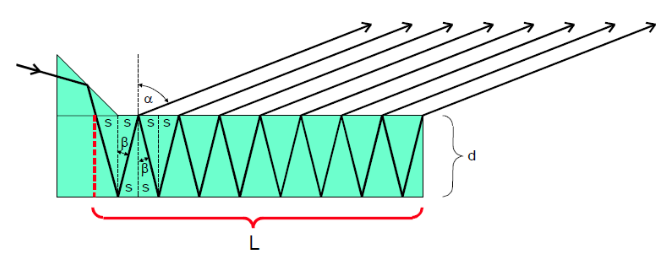
\includegraphics[scale=0.5]{pictures/lummergehrcke.png}
 \caption{Der Strahlengang in der Lummer-Gehrcke Platte. \cite{Versuchsbeschreibung}}
 \label{fig:lummergehrcke}
\end{figure}
\noindent
Über die Reflektion an jedem Prisma innerhalb der Platte verlässt ein Teil der
Strahlung die Platte. Jedes dieser Bündel kann dann konstruktiv interferieren
wenn die Bragg-Bedingung~\ref{eqn:bragg} erfüllt ist:
\begin{equation}
 2 n d \cos{\beta} = m \lambda.
 \label{eqn:bragg}
\end{equation}
\noindent
Hierbei bezeichnet $d$ die Dicke, $n$ den Brechungsindex der Platte, $m$ die
Ordnungszahl der Interferenz und $\lambda$ die eingestrahlte Wellenlänge. Wird nun
monochromatisches Licht in die Platte eingestrahlt, entspricht der
Gangunterschied der Strahlen der eingestrahlten Wellenlänge. Diese Messung ist
in einem Spektralbereich $\Delta \lambda_{D}$ möglich, wenn der Sinus des Austrittswinkels
genähert werden kann als $\sin{\alpha} \approx 1$. Dieser Spektralbereich wird auch als
Dispersionsgebiet bezeichnet und ist gegeben durch Gleichung~\ref{eqn:gebiet}\cite{Versuchsbeschreibung}:
\begin{equation}
 \Delta \lambda_{D} = \frac{\lambda^{2}}{2d} \frac{1}{\sqrt{n^{2}-1}}.
 \label{eqn:gebiet}
\end{equation}
Diese Einschränkung ist darin begründet, dass sich sonst verschiedene
Interferenzordnungen überlagern würden. Daher ist der minimale messbare
Unterschied zwischen zwei aufgespaltenen Wellenlängen $\Delta \lambda_{D}$.
Die Lummer-Gehrcke Platte besitzt ein Auflösevermögen $A$, welches durch
ihre Länge $L$ sowie dem Brechungsindex $n$ und der eingestrahlten Wellenlänge
$\lambda$ beeinflusst wird. Es ist gegeben durch Gleichung~\ref{eqn:auflösung} \cite{Versuchsbeschreibung}:
\begin{equation}
 A = \frac{\lambda}{\Delta\lambda} = \frac{L}{\lambda}(n^{2}-1).
 \label{eqn:auflösung}
\end{equation}
Für die Breite der Aufspaltung $\delta\lambda$ gilt Gleichung~\ref{eqn:aufspaltung} \cite{Versuchsbeschreibung}:
\begin{equation}
 \delta \lambda = \frac{\delta s}{\Delta s} \Delta \lambda_{D}.
 \label{eqn:aufspaltung}
\end{equation}
Hierbei beschreibt $\Delta s$ den Abstand der nicht-aufgespaltenen Linien und $\delta s$
die Breite der Aufspaltung.

\subsection{Messung}
\label{Messung}
Die in diesem Versuch verwendete Cadmium-Lampe zeigt vor allem zwei gut erkennbare
Spektrallinien, eine rote ($\lambda = \SI{638.3}{\nano\meter}$) sowie eine
blaue Linie ($\lambda = \SI{480}{\nano\meter}$). Bei der roten Linie kann eine
Messung des normalen, bei der blauen Linie des anormalen Zeeman-Effektes durchgeführt
werden. Hierfür muss zuerst das Magnetfeld geeicht werden, indem eine Hall-Sonde zwischen
die Polschuhe gebracht und bei verschiedenen Einstellungen des Netzteils die sich
ergebende Magnetfeldstärke gemessen wird. Dann werden die Wellenlängenaufspaltungen
für mehrere Ordnungen der roten und blauen Linie gemessen. Bei der blauen Linie wird
sowohl die $\sigma$- als auch die $\pi$-Linie gemessen. Dabei wird der Magnet auf die in der
Versuchsvorbereitung berechneten Werte eingestellt. Diese sind in
Tabelle~\ref{tab:magnet} abgebildet.
\begin{table}
  \centering
  \caption{Berechnete Werte für die benötigten Magnetfeldstärken.}
  \label{tab:magnet}
  \sisetup{table-format=1.2}
  \begin{tabular}{S S}
    \toprule
    {$g_{J}$} & {$B[T]$} \\
    \midrule
    1 & 0.68 \\
    2 & 0.31 \\
    1.5 & 0.42 \\
    0.5 & 1.25 \\
	\bottomrule
  \end{tabular}
\end{table}
